\section{Resultados}\label{sec:resultados}

Ao iniciar a página, o improvisador é colocado diante de emulador de terminal. Para obter ajuda de uso, o improvisador pode digitar $help$.
O comando \emph{Wavepot} pode ser executado com um argumento, que é o tamanho do \emph{buffer}.
Valores válidos devem ser potência de dois (2), entre 256 e 16384, sendo que o padrão é 1024 (ver Código \ref{code:resultado1}).
Alguns comando gerais como \emph{play}, \emph{stop}, \emph{pause} e \emph{reset} são utilizados para execução. 
\emph{Record} e \emph{export} para gravação de uma performance e exportação desta performance para um arquivo de extensão \emph{.wav}.

O comando \emph{play} inicia uma incrementação da variável $t$; o comando $pause$ "congela" $t$ e coloca o sintetizador em estado suspenso; $reset$ redefine $t=0$, porém não congela a incrementação. $Stop$ realiza a mesma tarefa que $pause$, porém desliga o sintetizador.

\begin{listing}
\begin{minted}[linenos,frame=lines,framesep=2mm,fontsize=\scriptsize]{javascript}
.........................................
. Virtual machine started at             .
. Thu Sep 03 2015 13:32:15 GMT-0300 (BRT).
. type help for instructions             .
..........................................
$\$$ wavepot 1024
..................................
. sintetizador de sample a sample. 
. amostragem: 44100              .
. canais: 2                      .
. buffer: 1024                   .
..................................
wavepot > play
wavepot > sin 440, 0.5
true
\end{minted}
\caption{Console do \emph{wavepot} aguardando dados de entrada do improvisador.}
\label{code:resultado1}
\end{listing}

\subsection*{Realizando sínteses}

A síntese no ambiente \emph{wavepot} é realizada fornecendo uma função que retorne dados entre -1.0 e 1.0, atuando diretamente sobre a linha 8 do exemplo apresentado na Seção \ref{sec:webaudioapi}.
No exemplo apresentado no Código \ref{code:resultado7}, ao utilizar a expressão \verb|Math.random() * 2 - 1|, a cada intervalo de tempo $td=1/SR$ (taxa de amostragem), um novo número randômico é mapeado entre o intervalo permitido, resultando em um ruído branco.

Uma maneira de simplificar o cálculo de um ruído, é definí-lo em uma função, como no Código \ref{code:ex1}. 

Já existe no aplicativo uma função \verb|noise(a)|.
Porém, como o objetivo é demonstrar seu uso, exemplificamos o processo ainda no Código \ref{code:resultado7}.
Ao  utilizar o \emph{token} \verb|def|, definimos em tempo de execução uma função chamada \verb|ruidobranco(a)|.

\begin{figure}[ht!]
\begin{minted}[linenos,frame=lines,framesep=2mm,fontsize=\scriptsize]{javascript}
wavepot > Math.random() * 2 - 1
true
wavepot> 0
true
wavepot > def rb(a) (Math.random() * 2 - 1) * amplitude #Ruido branco [a-amplitude = {0..1.0} ]
true
wavepot > inspect rb
/*
 Ruido branco [a-amplitude = {0..1.0} ]
 */
var rb;

rb = function(a) {
  return a * (Math.random() * 2 - 1);
};
wavepot > rb(0.71)
true
wavepot > mute()
true
wavepot> rb 0.71
true
wavepot > stop
true
\end{minted}
\caption{Exemplo de código para produzir e definir um ruído branco.}
\label{code:resultado7}
\end{figure}

Uma característica emprestada do \emph{wavepot} é o encorajamento ao uso de comentários como forma de documentar as funções criadas pelo usuário.
No $Termpot$ são usados no final da definição da função, seguido do caracter \#, sem espaço inicial.

Para silenciar o sistema, três formas de codificação são possíveis.
Uma vez que o console aceita valores numéricos, ao digitar 0, ouvimos um silêncio.
Existe também a função \verb|mute()| pré-definida.
A terceira desliga o sistema.
As três maneiras estão demonstradas no Código \ref{code:resultado7}

% -------------------------------------------------------------------------------------------------
\subsection*{Utilização da variável $t$}

A utilização de uma variável que controla o tempo foi discutida brevemente no final da Seção \ref{sec:webaudioapi}.
No caso do $Termpot$ recorremos a uma supressão desta variável, como demonstrado no Código \ref{code:resultado14}, afim de atingir uma economia de caracteres.

\begin{listing}
\begin{minted}[linenos,frame=lines,framesep=2mm,fontsize=\scriptsize]{javascript}
wavepot > inspect tau
/* Ciclo Trigonometrico completo */
var tau = 2*Math.PI;
true
wavepot > Math.sin tau * 440 * t
true
wavepot > 0
true
wavepot > def senoide(f, a) (Math.sin tau * f * t) * a
senoide defined
wavepot > senoide 415, 0.5
true
\end{minted}
\caption{Exemplo de código do Wavepot sem o controle explicíto do tempo (t)}
\label{code:resultado14}
\end{listing}


A implementação acima foi possível como demonstrado na linha 48, e entre as linhas 105 e 138 no repositório git\footnote{Disponível em \url{https://github.com/jahpd/termpot/blob/master/wavepot-runtime.js}.}.

% -------------------------------------------------------------------------------------------------
\subsubsection*{Implementação estereofônica}

Até o momento, os recursos utilizados apenas retornam um áudio monofônico expandido para dois canais.
Todavia, há uma maneira simples de separar os canais, partindo da criação de uma função que aceite dois valores de entrada e retorne um Array de dois elementos, como demonstrado no Código \ref{code:resultado15}.

\begin{listing}
\begin{minted}[linenos,frame=lines,framesep=2mm,fontsize=\scriptsize]{javascript}
wavepot > def stereo(l, r) [l, r] #Retorna um audio stereo de 
quaisquer inputs
wavepot > inspect stereo
/*
Retorna um audio stereo de quaisquer inputs
 */
var stereo;

stereo = function(l, r) {
  return [l, r];
};
wavepot > stereo sin(440,0.5), sin(330, 0.5)
true
\end{minted}
\caption{Exemplo de código estereofônico do Wavepot}
\label{code:resultado15}
\end{listing}

% -----------------------------------------------
\subsection{Implementação de controles}

Conforme apresentado na Figura \ref{fig:termpot}, a GUI do Termpot possui do lado direito um painel; que pode ser utilizado como uma mesa de \emph{sliders}.
Desta forma, as interfaces gráficas controlam parâmetros de funções usadas.
Abaixo descrevemos o procedimento para criar um novo controle, ele mesmo uma função:

\begin{figure}[!h]
\centering
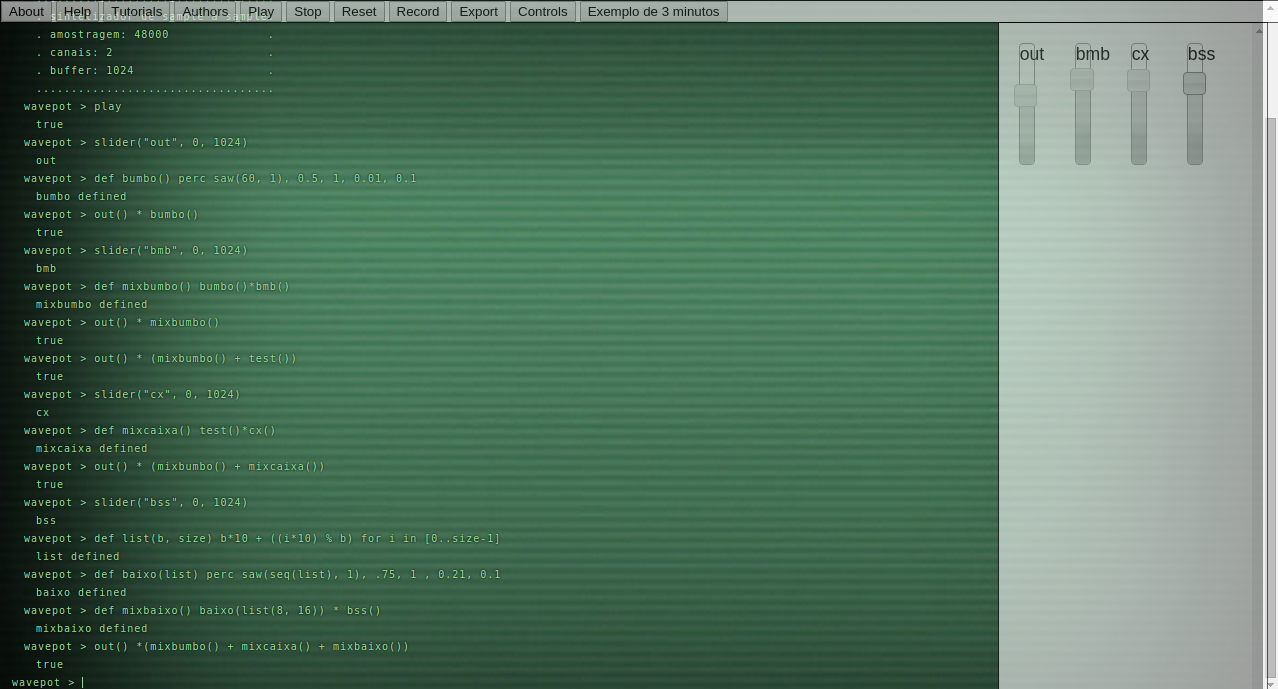
\includegraphics[scale=0.35]{termpot.png}
\caption{Aplicativo \emph{Termpot}. \textbf{Fonte}: autores.}
\label{fig:termpot}
\end{figure}

\begin{listing}
\begin{minted}[linenos,frame=lines,framesep=2mm,fontsize=\scriptsize]{javascript}
wavepot > slider("left", 0, 1024)
true
wavepot > slider("right", 0, 1024)
true
wavepot > stereo sin(440,0.5)*left(), sin(330, 0.5)*right()
true
\end{minted}
\caption{Exemplo de código do Wavepot}
\label{code:resultado15}
\end{listing}


